\chapter{ART Native Code Store}\label{chapter:native_code_store}

Since DEX code seems like to be the weak spot for Apps in terms of security
topics as well was for licensing and piracy issues, it seems logic to try
to circumvent this file format. When comparing the mobile device distribution
system of Apps to desktop environments like Linux, Windows or MacOS, it becomes
clear that the main difference is the distribution of Java like bytecode compared to binaries, at least for commercial software or the operating system itself. So the question would be if it is possible to establish an App store that only distributes native code instead of APKs. Like deduced in \autoref{section:app_execution_detail}, it is very likely that the DEX file is still needed for addressing native code inside of an ELF.
Still that thought experiment will be performed in order to clearify if it is possible in general.

At first, an architecture needs to be defined that would be suitable for an alternative native code App store. To keep the user experience as is, it would be beneficial to be able to still use the Google Play App Store for distributing Apps. Therefore at least a barebone APK for the application needs to be created that will then be placed into the Google Store.
That application can then be installed the common Android way. At its first startup, it then could connect to the actual native code app store
requesting the functional App in form of raw bytecode or an ELF file that
somehow gets injected in the current barebone application.
So the barebone version needs to implement at least the communication mechanism as well as the self modifying code part that can handle the receiving code snippets (\autoref{fig:native_store_arch} visually shows
the explained architecture).
\begin{figure}[htb]
  \centering
  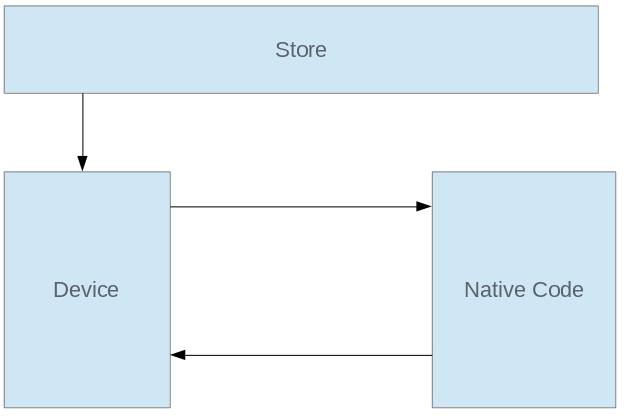
\includegraphics[scale=0.5]{figures/native_store_arch}
  \caption[Native Code Store Architecture]{Native Code Store Architecture}
  \label{fig:native_store_arch}
\end{figure}
When assuming that no root rights are present, the possibilities of injecting code and changing files are of course very limited. Remember that there do exist
two identical DEX files after the installation process, one DEX inside of the original \code{base.apk} package and one embedded inside of the \code{dex2oat}
output (ELF file). 

